\noindent

\includegraphics[height=1.25cm]{images/pictograms/replication}
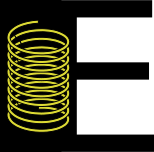
\includegraphics[height=1.25cm]{images/pictograms/elasticity}

\includegraphics[height=1.25cm]{images/pictograms/benchmark}

\includegraphics[height=1.25cm]{images/pictograms/triangle}

\includegraphics[height=1.25cm]{images/pictograms/under_construction}

\includegraphics[height=1.25cm]{images/pictograms/FEM}

\includegraphics[height=1.25cm]{images/pictograms/paraview}

%%%%%%%%%%%%%%%%%%%%%%%%%%%%%%%%%%%%%%%%%%%%%%%%%%%%%%%%%%%%%%%%%%%%%%%%%%%%%%%%%%%%%%%%%%%%%%%%%%%

\begin{flushright} {\tiny {\color{gray} python\_codes/fieldstone\_179/text.tex}} \end{flushright}

%\lstinputlisting[language=bash,basicstyle=\small]{python_codes/template_keywords.key}

\par\noindent\rule{\textwidth}{0.4pt}

\begin{center}
\inpython
{\small Code: \url{https://github.com/cedrict/fieldstone/tree/master/python_codes/fieldstone_179}}
\end{center}

\par\noindent\rule{\textwidth}{0.4pt}

Last revision: August 18th, 2025.

\par\noindent\rule{\textwidth}{0.4pt}

%%%%%%%%%%%%%%%%%%%%%%%%%%%%%%%%%%%%%%%%%%%%%%%%%%%%%%%%%%%%%%%%%%%%%%%%%%%%%%%%%%%%%%%%%%%%%%%%%%%

This \stone is inspired by \textcite{koko07} (2007) in which the author presents 
a clever way to build and assemble elemental matrices for a 2d $P_1$ elastic code.
The 'clever' way is presented in Section~\ref{MMM-ss:p1}.

%------------------------------------------------
\section*{The physical problem}

The domain $\Omega$ is described by the polygon
$(-1,-1), (0,-2), (2, 0), (0, 2), (-1,+1), (0, 0)$.

The exact solution is known in polar coordinates $(r,\theta)$:
\begin{eqnarray}
u_r(r,\theta)
&=&\frac{1}{2\mu} r^\alpha 
[(c_2 - \alpha - 1)c_1 \cos((\alpha - 1)\theta) 
- (\alpha + 1) \cos((\alpha + 1)\theta)] \nn\\
u\theta(r,\theta)&=& 
\frac{1}{2\mu}
[(\alpha + 1) \sin((\alpha + 1)\theta) 
+ (c_2 + \alpha - 1)c_1 \sin((\alpha - 1)\theta)]
\end{eqnarray}
The exponent $\alpha$ is the solution of the equation
\[
\alpha \sin(2\omega) + \sin(2\omega \alpha ) = 0
\]
with $\omega=3\pi/4$ and
\[
c_1 = -\frac{\cos((\alpha+1)\omega)}{\cos((\alpha-1)\omega)}
\qquad
c_2 = 2 \frac{\lambda + 2\mu}{\lambda+\mu}
\]


The displacement field are solution of the momentum equation 
with $\vec{f} = \vec{0}$ and $u_D = (u_r , u_\theta )$ on 
$\Gamma = \Gamma_D$ . Numerical
experiments are carried out with Young’s modulus E = 100000 and Poisson’s coefficient $\nu$ = 0.3. The magnitude of
the gradient $|\vec\nabla \vec{u}|$ of the exact solution 
has a singularity at the re-entrant corner $(0,0)$. This singularity,
despite being very local, is a significant source of error.

%------------------------------------------------
\section*{Implementation}




%------------------------------------------------
\section*{Results}

\begin{center}
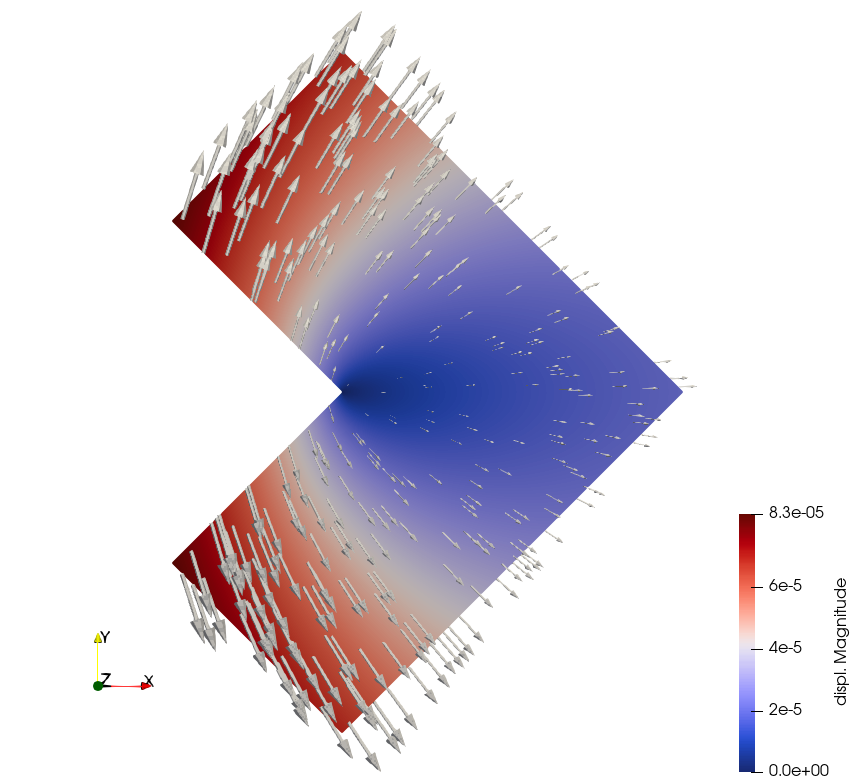
\includegraphics[width=7cm]{python_codes/fieldstone_179/RESULTS/disp}
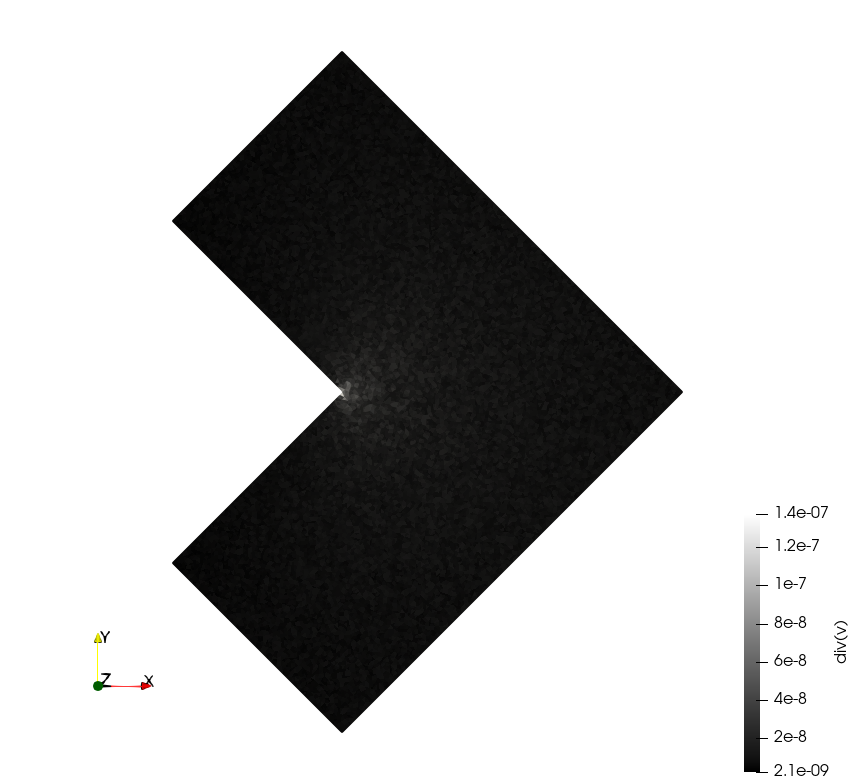
\includegraphics[width=7cm]{python_codes/fieldstone_179/RESULTS/divv}\\
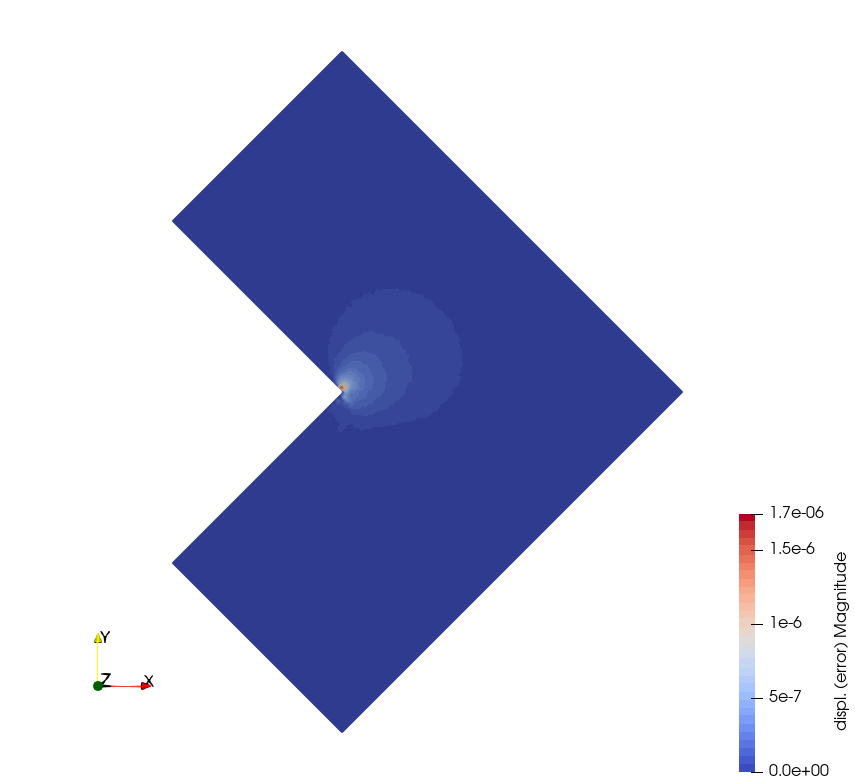
\includegraphics[width=7cm]{python_codes/fieldstone_179/RESULTS/error}
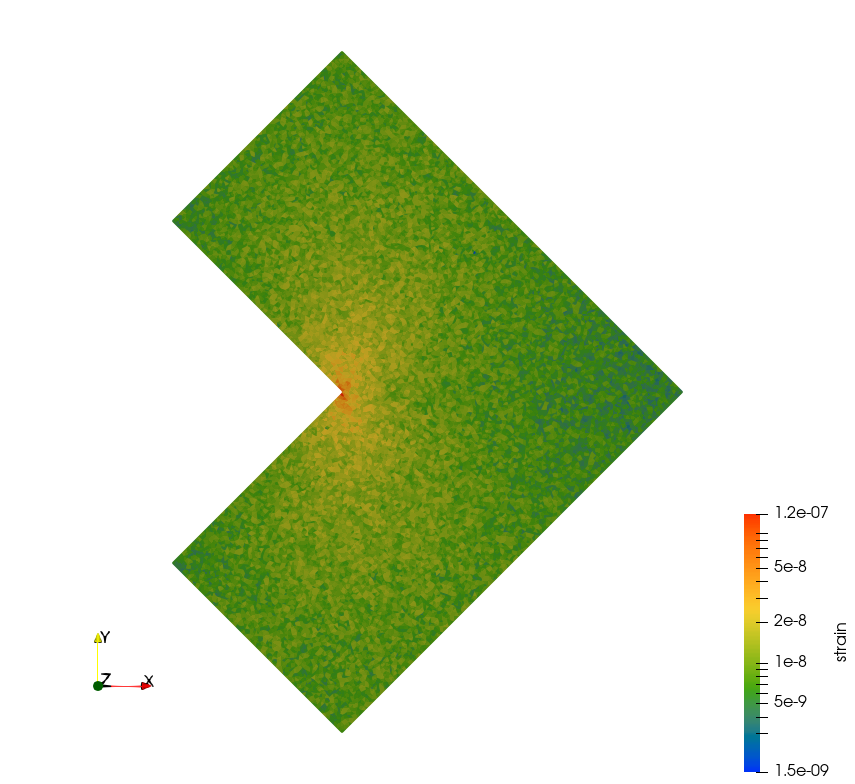
\includegraphics[width=7cm]{python_codes/fieldstone_179/RESULTS/strain}
\end{center}


\begin{center}
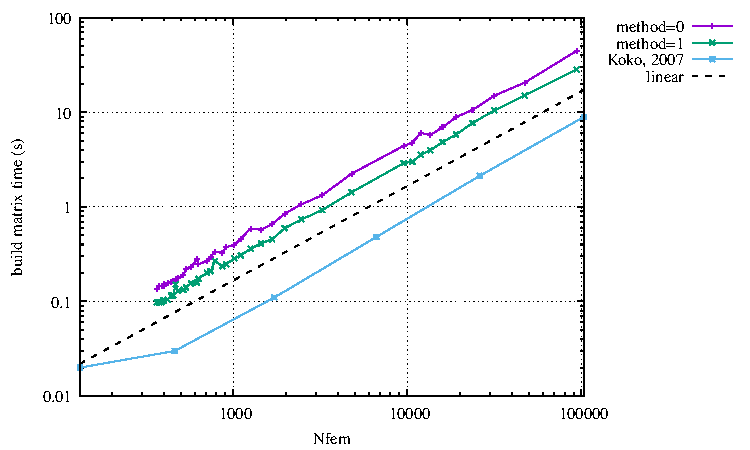
\includegraphics[width=8cm]{python_codes/fieldstone_179/RESULTS/build.pdf}
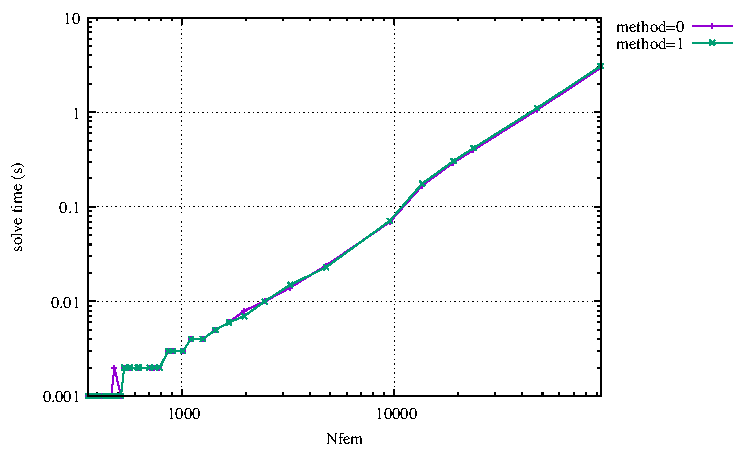
\includegraphics[width=8cm]{python_codes/fieldstone_179/RESULTS/solve.pdf}
\end{center}


